% Options for packages loaded elsewhere
\PassOptionsToPackage{unicode}{hyperref}
\PassOptionsToPackage{hyphens}{url}
%
\documentclass[
  english,
  man]{apa6}
\usepackage{amsmath,amssymb}
\usepackage{lmodern}
\usepackage{ifxetex,ifluatex}
\ifnum 0\ifxetex 1\fi\ifluatex 1\fi=0 % if pdftex
  \usepackage[T1]{fontenc}
  \usepackage[utf8]{inputenc}
  \usepackage{textcomp} % provide euro and other symbols
\else % if luatex or xetex
  \usepackage{unicode-math}
  \defaultfontfeatures{Scale=MatchLowercase}
  \defaultfontfeatures[\rmfamily]{Ligatures=TeX,Scale=1}
\fi
% Use upquote if available, for straight quotes in verbatim environments
\IfFileExists{upquote.sty}{\usepackage{upquote}}{}
\IfFileExists{microtype.sty}{% use microtype if available
  \usepackage[]{microtype}
  \UseMicrotypeSet[protrusion]{basicmath} % disable protrusion for tt fonts
}{}
\makeatletter
\@ifundefined{KOMAClassName}{% if non-KOMA class
  \IfFileExists{parskip.sty}{%
    \usepackage{parskip}
  }{% else
    \setlength{\parindent}{0pt}
    \setlength{\parskip}{6pt plus 2pt minus 1pt}}
}{% if KOMA class
  \KOMAoptions{parskip=half}}
\makeatother
\usepackage{xcolor}
\IfFileExists{xurl.sty}{\usepackage{xurl}}{} % add URL line breaks if available
\IfFileExists{bookmark.sty}{\usepackage{bookmark}}{\usepackage{hyperref}}
\hypersetup{
  pdftitle={Cognitive Music Listening Space: A Multivariate Approach},
  pdfauthor={Brendon Mizener1, Mathilde Vandenberghe2, Herve Abdi1, \& Sylvie Chollet2},
  pdflang={en-EN},
  pdfkeywords={keywords},
  hidelinks,
  pdfcreator={LaTeX via pandoc}}
\urlstyle{same} % disable monospaced font for URLs
\usepackage{graphicx}
\makeatletter
\def\maxwidth{\ifdim\Gin@nat@width>\linewidth\linewidth\else\Gin@nat@width\fi}
\def\maxheight{\ifdim\Gin@nat@height>\textheight\textheight\else\Gin@nat@height\fi}
\makeatother
% Scale images if necessary, so that they will not overflow the page
% margins by default, and it is still possible to overwrite the defaults
% using explicit options in \includegraphics[width, height, ...]{}
\setkeys{Gin}{width=\maxwidth,height=\maxheight,keepaspectratio}
% Set default figure placement to htbp
\makeatletter
\def\fps@figure{htbp}
\makeatother
\setlength{\emergencystretch}{3em} % prevent overfull lines
\providecommand{\tightlist}{%
  \setlength{\itemsep}{0pt}\setlength{\parskip}{0pt}}
\setcounter{secnumdepth}{-\maxdimen} % remove section numbering
% Make \paragraph and \subparagraph free-standing
\ifx\paragraph\undefined\else
  \let\oldparagraph\paragraph
  \renewcommand{\paragraph}[1]{\oldparagraph{#1}\mbox{}}
\fi
\ifx\subparagraph\undefined\else
  \let\oldsubparagraph\subparagraph
  \renewcommand{\subparagraph}[1]{\oldsubparagraph{#1}\mbox{}}
\fi
% Manuscript styling
\usepackage{upgreek}
\captionsetup{font=singlespacing,justification=justified}

% Table formatting
\usepackage{longtable}
\usepackage{lscape}
% \usepackage[counterclockwise]{rotating}   % Landscape page setup for large tables
\usepackage{multirow}		% Table styling
\usepackage{tabularx}		% Control Column width
\usepackage[flushleft]{threeparttable}	% Allows for three part tables with a specified notes section
\usepackage{threeparttablex}            % Lets threeparttable work with longtable

% Create new environments so endfloat can handle them
% \newenvironment{ltable}
%   {\begin{landscape}\begin{center}\begin{threeparttable}}
%   {\end{threeparttable}\end{center}\end{landscape}}
\newenvironment{lltable}{\begin{landscape}\begin{center}\begin{ThreePartTable}}{\end{ThreePartTable}\end{center}\end{landscape}}

% Enables adjusting longtable caption width to table width
% Solution found at http://golatex.de/longtable-mit-caption-so-breit-wie-die-tabelle-t15767.html
\makeatletter
\newcommand\LastLTentrywidth{1em}
\newlength\longtablewidth
\setlength{\longtablewidth}{1in}
\newcommand{\getlongtablewidth}{\begingroup \ifcsname LT@\roman{LT@tables}\endcsname \global\longtablewidth=0pt \renewcommand{\LT@entry}[2]{\global\advance\longtablewidth by ##2\relax\gdef\LastLTentrywidth{##2}}\@nameuse{LT@\roman{LT@tables}} \fi \endgroup}

% \setlength{\parindent}{0.5in}
% \setlength{\parskip}{0pt plus 0pt minus 0pt}

% \usepackage{etoolbox}
\makeatletter
\patchcmd{\HyOrg@maketitle}
  {\section{\normalfont\normalsize\abstractname}}
  {\section*{\normalfont\normalsize\abstractname}}
  {}{\typeout{Failed to patch abstract.}}
\patchcmd{\HyOrg@maketitle}
  {\section{\protect\normalfont{\@title}}}
  {\section*{\protect\normalfont{\@title}}}
  {}{\typeout{Failed to patch title.}}
\makeatother
\shorttitle{Music Descriptor Space}
\keywords{keywords\newline\indent Word count: X}
\DeclareDelayedFloatFlavor{ThreePartTable}{table}
\DeclareDelayedFloatFlavor{lltable}{table}
\DeclareDelayedFloatFlavor*{longtable}{table}
\makeatletter
\renewcommand{\efloat@iwrite}[1]{\immediate\expandafter\protected@write\csname efloat@post#1\endcsname{}}
\makeatother
\usepackage{lineno}

\linenumbers
\usepackage{csquotes}
\usepackage{caption}
\ifxetex
  % Load polyglossia as late as possible: uses bidi with RTL langages (e.g. Hebrew, Arabic)
  \usepackage{polyglossia}
  \setmainlanguage[]{english}
\else
  \usepackage[main=english]{babel}
% get rid of language-specific shorthands (see #6817):
\let\LanguageShortHands\languageshorthands
\def\languageshorthands#1{}
\fi
\ifluatex
  \usepackage{selnolig}  % disable illegal ligatures
\fi
\newlength{\cslhangindent}
\setlength{\cslhangindent}{1.5em}
\newlength{\csllabelwidth}
\setlength{\csllabelwidth}{3em}
\newenvironment{CSLReferences}[2] % #1 hanging-ident, #2 entry spacing
 {% don't indent paragraphs
  \setlength{\parindent}{0pt}
  % turn on hanging indent if param 1 is 1
  \ifodd #1 \everypar{\setlength{\hangindent}{\cslhangindent}}\ignorespaces\fi
  % set entry spacing
  \ifnum #2 > 0
  \setlength{\parskip}{#2\baselineskip}
  \fi
 }%
 {}
\usepackage{calc}
\newcommand{\CSLBlock}[1]{#1\hfill\break}
\newcommand{\CSLLeftMargin}[1]{\parbox[t]{\csllabelwidth}{#1}}
\newcommand{\CSLRightInline}[1]{\parbox[t]{\linewidth - \csllabelwidth}{#1}\break}
\newcommand{\CSLIndent}[1]{\hspace{\cslhangindent}#1}

\title{Cognitive Music Listening Space: A Multivariate Approach}
\author{Brendon Mizener\textsuperscript{1}, Mathilde Vandenberghe\textsuperscript{2}, Herve Abdi\textsuperscript{1}, \& Sylvie Chollet\textsuperscript{2}}
\date{}


\authornote{

Add complete departmental affiliations for each author here. Each new line herein must be indented, like this line.

Enter author note here.

The authors made the following contributions. Brendon Mizener: Stimuli creation, Survey design \& creation, Data collection \& processing, Statistical analyses, Writing - Original draft preparation; Mathilde Vandenberghe: Original concept, Survey design \& creation; Herve Abdi: Writing - Review \& Editing, Statistical guidance; Sylvie Chollet: Original concept.

Correspondence concerning this article should be addressed to Brendon Mizener, 800 W. Campbell Rd., Richardson Tex. E-mail: \href{mailto:bmizener@utdallas.edu}{\nolinkurl{bmizener@utdallas.edu}}

}

\affiliation{\vspace{0.5cm}\textsuperscript{1} University of Texas at Dallas\\\textsuperscript{2} YNCREA}

\abstract{
This is my abstract
}



\begin{document}
\maketitle

\begin{verbatim}
## [1] "It is estimated that your iterations will take 0.67 minutes."
## [1] "R is not in interactive() mode. Resample-based tests will be conducted. Please take note of the progress bar."
## ================================================================================
\end{verbatim}

Music listening is a complex cognitive activity that involves many judgments per second. Listeners continuously evaluate incoming information and compare it with that which came before. These judgments involve many different dimensions of music related to both the technical and affective aspects of this acoustic medium. Generally, however, in the literature, many researchers describe sound in only two dimensions; pitch and loudness (\textbf{Wallmark2019?}). Even music cognition researchers resort to isolating only one or two dimensions, such as pitch or rhythm (e.g., (\textbf{Krumhansl2000?})). Although the use of more realistic stimuli has become more common {[}citation{]}, researchers still tend to simplify stimuli so that they are isochronic or simplified in other ways. Additionally, performing traditional hypothesis testing in experiments that evaluate multiple dimensions quickly becomes cumbersome and inelegant, and it can be difficult to interpret results. Imaging studies, which have merit in their own right, similarly lack inclusion and require prohibitive amounts of resources, and are severely location-dependent. The gradual increase in complexity of behavior and cognition studies, coupled with the rise of questions about the universality of experience and the democratization of science, compels us to find novel ways of investigating the experience of music.\\
Another consistent limitation is population. In general, studies of this sort are limited to WEIRD people (Western, Educated, Industrialized, Rich, and Democratic), and also tend to lack representation in ethnic minority communities. By developing investigative paradigms that are accessible on mobile platforms, and that reduce participant demand as much as possible while maintaining rigor, we are likely to be able to reach a much greater subset of the population. If we are able to pair this kind of data gathering with appropriate exploratory analysis, we can target much more effectively where we might investigate with more traditional hypothesis testing.
The initial motivation for this paper was as precursor work to a study aimed at evaluating the cross-modal similarities between gustatory perception and auditory perception. While there exist various established gustatory `spaces' onto which music perception might be mapped, for example in wine tasting {[}wine citations here{]}, there is no similar space for music. The goal of this study was to evaluate whether or not there is a similar music perception space against which other sensory domains could be compared, and to select stimuli that could anchor the corners of such a space.

There is some previous work that has approached timbre specifically from a similar analytical perspective.

The current study aimed to evaluate a set of musical stimuli in two ways, by association with a list of adjectives, and by rating on a set of musical qualities. These will then be analyzed independently and then combined to see what effects can be deduced from the combination of the two.

Valence/arousal model

\begin{itemize}
\item
  as questions become more complex, the burden on researchers to define parameters in which to test and evaluate their results becomes much greater. Controlling for extraneous variables becomes a problem in and of itself.
\item
  lacks generalizability because of narrowness
\item
  rising question of universalities \& cross-cultural perception in music
\item
  how do we access a larger population
\item
  This all results in a need for an experimental paradigm that is robust to violations in experimental procedure, accesses
\end{itemize}

\hypertarget{cata-paradigm}{%
\subsection{CATA paradigm}\label{cata-paradigm}}

While not invented by (\textbf{Katz1933?}), the Check-All-That-Apply (CATA) investigative paradigm was used in that study to evaluate racial stereotypes among college students. As an method it's not terribly common in the psychological sciences any more, but it has been and continues to be used widely to ``obtain rapid product profiles'' (\textbf{Meyner2014?}) from participants. It is also commonly used in sensory evaluation. In this method, participants are asked to select any and all adjectives from a list that describe a given stimulus. This allows researchers to collect a lot of data about a given stimulus without placing demand on the participants. The onus is then on the researchers to aggregate and evaluate this data to see what insights may be gained on the stimuli. Because of the

\begin{itemize}
\tightlist
\item
  what it is (cite Katz \& Braly 1933, Meyners \& Castura)

  \begin{itemize}
  \tightlist
  \item
    Often used in sensory discrimination, consumer product research
  \item
    participant is instructed to select any and all qualities or descriptors that they associate with the presented stimulus.
  \end{itemize}
\item
  why is it good/how does it solve the problem

  \begin{itemize}
  \tightlist
  \item
    easy
  \item
    low demand
  \item
    robust to outlying responders
  \end{itemize}
\item
  why is it specifically useful for this paradigm (internet/online research)

  \begin{itemize}
  \tightlist
  \item
    Using a technique that minimizes participant effort while allowing for meaningful data gathering, in a context that necessitates data gathering from a distance
  \end{itemize}
\item
  what the data look like

  \begin{itemize}
  \tightlist
  \item
    After cleaning and preprocessing, the data for each participant will take the form of a pseudo contingency table. The difference here is that a contingency table is specifically when a participant selects only one option from a list for each stimulus, resulting in a table with one and only one one (1) per row. Because we are using the CATA technique, a one (1) at the intersection of each row or column indicates that the participant selected that adjective or musical quality for that stimulus. A zero means that they did not. These individual tables are all compiled into a `brick,' or three-dimensional array of data with Observations (stimuli) on the rows, variables (musical qualities or adjectives) on the columns, and participants on the third dimension, which we will refer to as `pages' here. This brick is then summed across pages into a single table, so that any given cell contains the total number of times a participant selected a given adjective or quality to match with a stimulus.
    From this point there are two sets of data that can be analyzed. The first is the 3D array, which can be analyzed using various distance analyses, to evaluate differences between the participants using grouping variables extracted from the demographics surveys. The other is the pseudo contingency table, which can be analyzed using various multivariate techniques.
  \end{itemize}
\item
  what processing steps are needed
\end{itemize}

\hypertarget{present-questions-methods-of-analysis}{%
\subsection{Present questions \& methods of analysis}\label{present-questions-methods-of-analysis}}

The initial motivation for this study came from a cross-modal study investigating the co-\_\_\_\_\_ between gustation perception, specifically beer, and music perception. Initial studies suggest that a wide variety in musical stimuli was necessary to determine any correlations or differences. As such, this study is designed to investigate whether a music cognitive listening space can be established using this paradigm to allow cross-modal comparison. Additional questions arise from the study itself: are there significant differences in how participants from different nationalities (and by extension musical cultures) perceive, or, more precisely, describe music? Are there parallels in how music non-specific descriptors and music-specific qualities are assigned to stimuli or evaluated?
To analyze the data collected here,
is there a cognitive space that can be deduced using this paradigm?
- Is that cognitive space robust across nationalities (i.e., musical cultures)
- Are there parallels between the ways that music is rated using music-specific dimensions \& adjectives
- To analyze this data, we use hypothesis free multivariate analyses paired with inference methods like the bootstrap (resampling) and the permutation test (randomization). Although the analyses do not specifically test hypotheses in the same way an ANOVA or t test would, these inferences methods allow us to draw conclusions about statistical significance from them.
- Correspondence analysis
- brick excerpts (stimuli)/descriptors/subjects
- pseudo contingency table
-
- PLSC
- 2 contingency tables (2 data tables)

\hypertarget{arousalvalence-modelother-models}{%
\subsubsection{Arousal/valence model/other models?}\label{arousalvalence-modelother-models}}

\begin{itemize}
\tightlist
\item
  What is it?
\item
  previous work on cognitive space in music perception
\end{itemize}

\hypertarget{where-we-got-the-words}{%
\subsubsection{Where we got the words}\label{where-we-got-the-words}}

\begin{itemize}
\item
  revisit the IRB application
\item
\end{itemize}

\hypertarget{multivariate-methods}{%
\subsection{Multivariate methods?}\label{multivariate-methods}}

\hypertarget{methods}{%
\section{Methods}\label{methods}}

\hypertarget{participants}{%
\subsection{Participants}\label{participants}}

Participants for this study were recruited in multiple ways, all of which represent convenience sampling. The participants in the United States were recruited using the traditional method of offering experimental participation credit, and also via social media. French participants were recruited by word of mouth, email, and social media. The only restrictions on participation were that the participant must have self-reported normal hearing. We recognize that although we suggest that data collected in this way have a much greater hypothetical reach, the data here represent a) a convenience sample, b) that is limited to participants that have access to the internet. Both of these specific limitations could be remedied when designing and implementing future research.\\
In addition to the convenience sample described above, We sought out a specific population with ten years or more of music training to evaluate the stimuli on explicitly musical dimensions. We recruited this population for two reasons: firstly, as a validation step, to ascertain whether the stimuli truly reflected the composer's intent. Secondly, we had the goal of evaluating how the musical qualities of the stimuli, as evaluated by the trained participants, correlated with the adjectives selected by those who participated in the adjectives survey.
All recruitment measures were approved by the UT Dallas IRB.

\hypertarget{material}{%
\subsection{Material}\label{material}}

\hypertarget{surveys}{%
\subsubsection{Surveys}\label{surveys}}

There were two separate surveys presented to participants. One evaluated the musical stimuli on concrete musical qualities like meter and genre, the other evaluated the stimuli using adjectives, and used the CATA paradigm. Both surveys also captured participants' demographic data, including age, gender, nationality, occupation, and musical experience. The musically trained participants completed the musical qualities survey (QS). The adjectives survey (AS) was administered without respect to participants' musical training. As a result, there is a wide range of musical experience present in the sample.
The words for the AS were selected using (\textbf{Wallmark2019?}) as a guide and in consult with a French professional musician. Some words were initially selected in French and some in English. In all cases, words were selected for which there was a clear French (vis-a-vis English) translation. The words and their translations are listed in {[}supplementary materials?{]}. The qualities assessed in the QS were selected from standard music-theoretical descriptors of music. For example, when rating the excerpts on tempo, participants were asked to rate the excerpt using the scale \emph{Very Slow}, \emph{Slow}, \emph{Moderately Slow}, \emph{Moderate}, \emph{Moderately Fast}, \emph{Fast}, and \emph{Very Fast}. The full list of musical qualities and associated levels is in {[}supplementary materials?{]}.

\hypertarget{stimuli}{%
\subsubsection{Stimuli}\label{stimuli}}

All stimuli were original stimuli composed for this study. They were designed to evaluate a number of musical dimensions and control for others (e.g., timbre). The stimuli were all string quartets, in order to control for the confounding factor that different instruments are fundamentally described in different ways. All stimuli were between 27s and 40s long, with an average length of 32.4s. The intent was to have all stimuli be around 30s long while preserving musical integrity. All stimuli were composed between April 13 and June 18, 2020.

\hypertarget{procedure}{%
\subsection{Procedure}\label{procedure}}

Participants were provided with a link to either the AS or the QS. Both surveys were administered using Qualtrics. After standard informed consent, participants were instructed to listen to the excerpts presented either using headphones or in a quiet listening environment. Participants in the AS condition answered a single question per excerpt, in which they selected any and all adjectives that they felt described the excerpt. Participants in the QS condition answered 10 questions per excerpt, rating the excerpts using the qualities and scales provided.

\hypertarget{data-analysis}{%
\subsection{Data analysis}\label{data-analysis}}

Raw data were cleaned and processed in Excel and R. This included translating all French responses to English for ease of analysis. Data were cleaned and transformed into a pseudo contingency table for each participant. These individual tables were all compiled into into two `bricks,' or three-dimensional arrays of data with Observations (stimuli) on the rows, variables (musical qualities or adjectives) on the columns, and participants on the third dimension, which we will refer to as `pages' here. Each array was then summed across pages into a single table, so that any given cell contained the total number of times a participant selected a given adjective or quality for a given stimulus.
The arrays were analyzed using distance analyses to evaluate differences between the participants using grouping variables extracted from the demographics surveys. The summed tables were analyzed using Correspondence Analysis. Since we did not use \emph{a priori} grouping variables for the excerpts, the summed tables were evaluated using hierarchical cluster analyses to see what groupings arose during evaluation.
A final analysis (Partial Least Squares Correlation, PLSC) evaluated correlations between the two summed data tables to see what information was shared between the two tables.
For each of these analyses, variance is extracted in the form of eigenvalues, which form the principal components of the maps shown below. The dimensions extracted in this process are by definition orthogonal and share no information. For each of the analyses below, we focus on the first two dimensions. Third dimensions are presented solely for the sake of illustration.

\hypertarget{correspondence-analysis}{%
\subsubsection{Correspondence Analysis}\label{correspondence-analysis}}

Correspondence Analysis (CA) is similar to Principal Components Analysis (PCA), except that it allows for the analysis of qualitative data. Because of the organization of the data, this technique allows for a biplot of both rows and columns in a single factor space. We can also calculate and identify which observations (stimuli) or variables (adjectives or qualities) contribute significantly to a given dimension in the factor space. In addition to factor plots, we used permutation tests and bootstrapping to project confidence intervals for the means of certain variables in the factor spaces, which allows for statistical inferences.

\hypertarget{partial-least-squares-correlation}{%
\subsubsection{Partial Least Squares Correlation}\label{partial-least-squares-correlation}}

Partial Least Squares Correlation (PLSC) is analyzes two data tables either on the same observations (rows) or variables (columns). In this case, the stimuli. This technique is commonly used in imaging studies to evaluate correlations between matrices of imaging data and of behavioral or task data. In this technique, we will be looking at covariance and correlation between the variables in the two tables.

\hypertarget{results}{%
\section{Results}\label{results}}

\hypertarget{experiment-1-musical-qualities-survey}{%
\subsection{Experiment 1: Musical Qualities Survey}\label{experiment-1-musical-qualities-survey}}

\hypertarget{participants-1}{%
\subsubsection{Participants}\label{participants-1}}

The scree plot below shows the eigenvalues for the distance analysis between musical experts. The usual guideline of analyzing only dimensions with eigenvalues greater than one seems prohibitive here, as all dimensions except the last have \(\lambda\) \textgreater{} 1. For the purposes of this experiment, we've opted to focus on the first two dimensions, with \(\lambda\) = 9.36 and \(\lambda\) = 7.98, respectively. This analysis revealed no significant difference between the experts when grouped either by nationality or by gender identity. Training level was not considered as a factor for this analysis because this survey was only distributed to participants with greater than 10 years of musical training.

\begin{figure}

{\centering 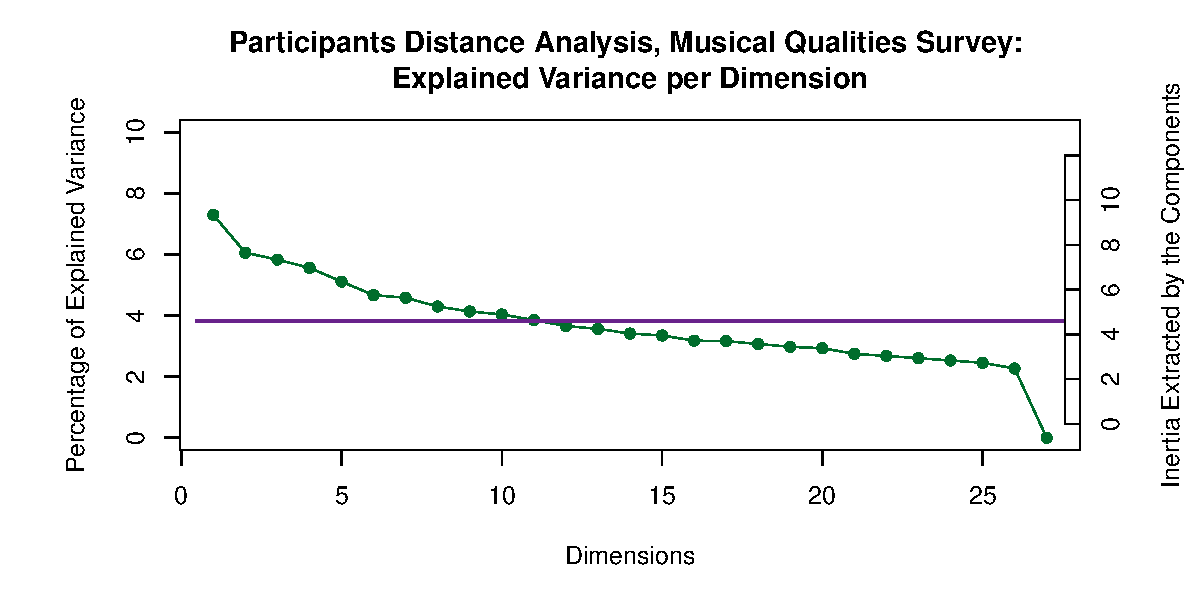
\includegraphics{Music-Descriptor-Space_files/figure-latex/screeRV-1} 

}

\caption{ }\label{fig:screeRV}
\end{figure}

\hypertarget{excerpts}{%
\subsubsection{Excerpts}\label{excerpts}}

\begin{itemize}
\tightlist
\item
  first three dimensions explain \textasciitilde40\% of variance

  \begin{itemize}
  \tightlist
  \item
    first two explain \textasciitilde30\% of variance (find which elements contribute the most, display in table?)
  \item
    First dimension is dominated by tempo and articulation, and the loud and soft levels of the dynamics quality
  \item
    second dimension is dominated by meter and genre
  \item
    third dimension is dominated by jazz genre and harmony variables (this excerpt is an outlier), other significant contributions come from dynamics and density, and to a lesser extent some contour.
  \end{itemize}
\end{itemize}

\hypertarget{experiment-2-musical-adjectives-survey}{%
\subsection{Experiment 2: Musical Adjectives Survey}\label{experiment-2-musical-adjectives-survey}}

\hypertarget{participants-2}{%
\subsubsection{Participants}\label{participants-2}}

The distance analyses between participants in either survey revealed significant group differences between French and American participants in the AS.

\hypertarget{excerpts-1}{%
\subsubsection{Excerpts}\label{excerpts-1}}

\begin{itemize}
\tightlist
\item
  first three dimension account for \textasciitilde80\% of the variance. Both of the first two dimensions carry information from both the valence and arousal dimensions, suggesting that they aren't orthogonal.

  \begin{itemize}
  \tightlist
  \item
    first dimension explains 50+\%,

    \begin{itemize}
    \tightlist
    \item
      strong contributions in the positive direction are Sad, Dark, Melancholy, Slow, Mysterious, Solemn, Disturbing.
    \item
      strong contributions in the negative direction are Fast, Dancing, Happy, Colorful, and Bright.
    \end{itemize}
  \item
    Second dimension 20+\%

    \begin{itemize}
    \tightlist
    \item
      strong + contributions: Aggressive, Fast, Disturbing, Mysterious, Solemn, Complex
    \item
      strong - contributions: Warm, Soft, Slow, Happy, Round, Light.
    \end{itemize}
  \item
    The third and fourth dimensions may represent an eigenplane, suggesting two dimensions that are very closely related in variance extracted and information represented.
  \end{itemize}
\end{itemize}

\hypertarget{experiment-3-combined-surveys}{%
\subsection{Experiment 3: Combined Surveys}\label{experiment-3-combined-surveys}}

\hypertarget{participants-3}{%
\subsubsection{Participants}\label{participants-3}}

PLSC:
- The

\hypertarget{discussion}{%
\section{Discussion}\label{discussion}}

\begin{itemize}
\tightlist
\item
  Because of the nature of the CA, the musical qualities survey is not robust to outliers.
\item
  hierarchical clustering revealed that there are differences in groupings between the musical qualities and the adjectives judgments.
\item
  valence/arousal model is very clear in the adjectives data
\item
  which qualities dominate which dimensions in the musical qualities survey? Why? Is it because of clear subjective/objective agreement on some specific musical qualities?
\end{itemize}

\hypertarget{limitations-future-directions}{%
\subsection{Limitations \& future directions}\label{limitations-future-directions}}

\begin{itemize}
\tightlist
\item
  continue to evaluate more participants from more varying backgrounds
\item
  increase sample size between highly trained musicians and others
\item
  add more dimensions (melodic complexity)
\end{itemize}

\newpage

\hypertarget{references}{%
\section{References}\label{references}}

\begingroup
\setlength{\parindent}{-0.5in}
\setlength{\leftskip}{0.5in}

\hypertarget{refs}{}
\begin{CSLReferences}{0}{0}
\end{CSLReferences}

\endgroup


\end{document}
